\documentclass[10pt]{beamer}

\usepackage[utf8]{inputenc}
\usepackage[french]{babel}
\usepackage{amsfonts,amsmath,amssymb,bbold}
\usepackage{calrsfs}
\usepackage[lined,boxed, ruled,vlined, french]{algorithm2e}
\usepackage{multirow}
\usepackage{mathtools,mathptmx}
\usepackage{empheq}
\usepackage{enumerate}
\usepackage{makecell}

%% for images print :
\usepackage{svg}
\usepackage{tikz}
\usetikzlibrary{tikzmark,calc,arrows,shapes,decorations.pathreplacing}
\tikzset{every picture/.style={remember picture}}
\usepackage{accents}
\newcommand\myubar[1]{%
\underaccent{\bar}{#1}}

\usepackage{comment}

%%% theme of diapo

%\usetheme{PaloAlto}
\usecolortheme{seahorse}
%%%%title page
\defbeamertemplate*{title page}{customized}[1][]
{
    \begin{center}
    \usebeamerfont{title}\inserttitle\par
  %\usebeamerfont{subtitle}\usebeamercolor[fg]{subtitle}\insertsubtitle\par
    \vfill
      \begin{minipage}{0.3\textwidth}
        \begin{center} 
            
\includegraphics[width=.8\linewidth]{logos/logo_LBBE.png}
        \end{center}
    \end{minipage}
    \begin{minipage}{0.3\textwidth}
        \begin{center} 
            
\includegraphics[width=.8\linewidth]{logos/logo_UCBL.png}
        \end{center}
    \end{minipage}
    \begin{minipage}{0.3\textwidth}
        \begin{center} 
            
\includegraphics[width=.8\linewidth]{logos/inra_aggro.png}
        \end{center}
    \end{minipage}
    \vfill
    \insertauthor\par
    \insertdate\par
   \end{center}
  }
%%%%% footer
\defbeamertemplate*{footline}{my footline}
{
	\leavevmode%
	\hbox{%
		\begin{beamercolorbox}[wd=.3\paperwidth,ht=2.25ex,dp=1ex,center]{author in head/foot}%
			\usebeamerfont{author in head/foot}\insertshortauthor
		\end{beamercolorbox}%
		\begin{beamercolorbox}[wd=.6\paperwidth,ht=2.25ex,dp=1ex,center]{title in head/foot}%
			\usebeamerfont{title in head/foot}\insertshorttitle
		\end{beamercolorbox}%
		\begin{beamercolorbox}[wd=.1\paperwidth,ht=2.25ex,dp=1ex,center]{date in head/foot}%
			\insertframenumber{} / \inserttotalframenumber\hspace*{1ex}
	\end{beamercolorbox}}%
	\vskip 0pt%
    }
%\beamertemplatenavigationsymbolsempty


\title{Méthodes d'intégration de données pour la génomique en cellules uniques}
\author{Claire \textsc{GAYRAL}}% \\ Encadrée par Franck \textsc{Picard} et Julien \textsc{Chiquet}}
%\institute{Université Claude Bernard, Lyon 1}
\date{5 septembre 2019}


\begin{document}

\begin{frame}{}
    \frametitle{}
    {\huge Audition hors-concours E2M2}
    
    \titlepage
    
\end{frame}

\section{Le contexte : Séquençage en cellule unique}
\begin{frame}{}
    \begin{center}
        {\Huge Le contexte : }\\
        \vfill
        {\LARGE Séquençage en cellule unique}
    \end{center}
\end{frame}

\begin{frame}{Séquençage en cellule unique}
    
\end{frame}
\begin{frame}{Difficultés}
    \begin{minipage}[t]{0.48\linewidth}
    \uncover<1->{
    
    \begin{center} 
    Distribution des données \\ de comptage :
            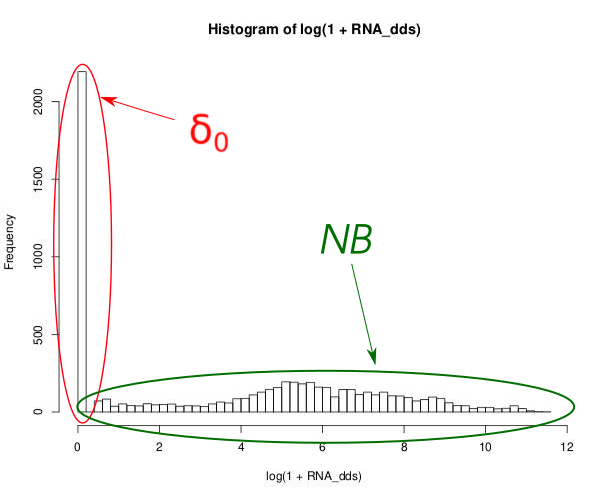
\includegraphics[height=0.40\textheight]{graphs/hist_all_genes_modif2.png}
        \end{center}
        $\rightarrow$ Modèle Négitive Binomiale Zero-Inflated  : $$ \boxed{ Y_{i}^g \sim \color{red}{\pi \delta_0} + \color{green}{(1-\pi) \, \mathcal{NB}(n,p) }}$$ 
    }
    \end{minipage}
    \begin{minipage}[t]{0.45\linewidth}
        \uncover<2->{
        Peu de mesures à disposition :\\
        
        $\rightarrow$ Intégrer des données issues de différentes manipulations \\
        
        $\rightarrow$ lskdnf
        }
    \end{minipage}
\end{frame}

\section{L'objet : Le sujet et les objectifs de la thèse}
\begin{frame}{}
    \begin{center}
        {\Huge L'objet : }\\
        \vfill
        {\LARGE Le sujet et les objectifs de la thèse}
    \end{center}
\end{frame}


\begin{frame}{Le sujet : Intégrer des jeux en cellule unique }
    Deux approches pour prendre en compte la distribution : 
    \begin{itemize}
        \item Adapter les modèles existants pour prendre en compte la distribution
        \item Corriger la distribution par une transformation statistique non linéaire 
    \end{itemize}
\end{frame}

\section{Les moyens : Les moyens pour réaliser cette thèse}
\begin{frame}{}
    \begin{center}
        {\Huge Les moyens : }\\
        \vfill
        {\LARGE Les moyens pour réaliser cette thèse}
    \end{center}
\end{frame}

\begin{frame}{Les moyens}
\begin{itemize}
    \item \textbf{Directeurs de thèse :} \\
        \begin{center}
        \begin{tabular}{ |c|c| } 
            \hline
            Franck Picard & Julien Chiquet \\
             \hline
             cell1 & cell1 \\ 
             cell2 & cell2 \\ 
             cell3 & cell3 \\ 
             \hline
        \end{tabular}
        \end{center}

    \item \textbf{Adéquation avec les laboratoires d'accueil : }\\
    \begin{center}
        \begin{tabular}{ |c|c| } 
            \hline
            LBBE (Lyon) & AgroParitech (Paris) \\
             \hline
             cell1 & cell1 \\ 
             cell2 & cell2 \\ 
             cell3 & cell3 \\ 
             \hline
        \end{tabular}
        \end{center}
    \item \textbf{Adéquation avec mon plan d'études :} \\
        \begin{itemize}
            \item Master en Mathématiques appliquées à la biologie
           % \item Année en BCPST
            \item Développement logiciel
            \item Stage M1 sur des traitement de données big data avec Sébastien Lousteau
            \item Stage M2 en bio-mathématiques sur des données en séquençage unique
        \end{itemize}
\end{itemize}
    
\end{frame}




\end{document}
